\documentclass[12pt]{article}
\usepackage{esqu1}
\pagestyle{fancy}

\lhead{Brandon Lin}
\chead{Multivariate Calculus}
\rhead{Fall 2015}

\begin{document}
\title{Multivariate Calculus}
\author{Brandon Lin\\Stuyvesant High School\\Fall 2015\\Teacher: Ms. Avigdor}
\maketitle
\newpage
\section*{Introduction}
These are the notes from the course I took at Stuyvesant High School, Fall 2015. Note: these are not the exact notes that were taken; these notes skip some properties that should be obvious if you took precalculus.
\section{3 Dimensional Space}
A \textbf{plane} can be represented by the equation $Ax + By + Cz + D = 0$. 
\begin{itemize}
\item When one of $A,B,C$ is nonzero, the plane is parallel to a \textbf{coordinate plane} (the $xy$-plane, $xz$-plane, or $yz$-plane).
\item When two of them are nonzero, the plane is paralle to a coordinate axis.
\item When all of them are nonzero, the plane intersects all three axes.
\end{itemize}

A \textbf{cylinder} is a surface that consists of all lines parallel to a given line and passing through a given curve. 

For example, a \textbf{right circular cylinder} can be represented by the equation $x^2 + (z-3)^2 = 4$. This cylinder has an axis of symmetry parallel to the $y$-axis, and has radius 2.

To graph an arbitrary surface/cylinder, we look at the \textbf{traces} that the surface makes with the coordinates planes and any planes parallel to the coordinate axes. The traces are the intersection between the two. For example, if we wish to look at the traces that the cylinder makes with the $xy$-plane, we let $z=0$ (the equation for the $xy$-plane) and see what equation that gives us on the plane. Likewise, to get the trace for any plane parallel to that $xy$-plane, we let $z=k$, and we find the intersection of the surface and the plane keeping $k$ constant.

\section{Vectors}
\subsection{Properties of Vectors}
\begin{itemize}
\item $\vec{u} + \vec{v} = \vec{v} + \vec{u}$ (Commutative)
\item $(\vec{u} + \vec{v}) + \vec{w} = \vec{u} + (\vec{v} + \vec{w})$ (Associative)
\item $\vec{u} + \vec{0} = \vec{0} + \vec{u} = \vec{u}$ (Identity Element under addition)
\item $\vec{u} + (-\vec{u}) = \vec{0}$ (Additive Inverse)
\item $c(\vec{u} + \vec{v}) = c\vec{u} + c\vec{v}$ (Distributive, vector)
\item $(c+d)\vec{u} = c\vec{u} + d\vec{u}$ (Distributive, scalar)
\item $c(d\vec{u}) = (cd)\vec{u}$ (Mixed Associative)
\item $1\vec{u} = \vec{u}$ (Identity Element)
\end{itemize}

\subsection{The Dot/Scalar Product}
If $\vec{u} = \la u_1, u_2, \dots, u_n \ra$ and $\vec{v} = \la v_1, v_2, \dots, v_n \ra$, then \[ \vec{u} \cdot \vec{v} = u_1v_1 + u_2v_2 + \cdots + u_nv_n = \sum_{i = 1}^n{u_iv_i} \]
\begin{figure}[h!]
\centering
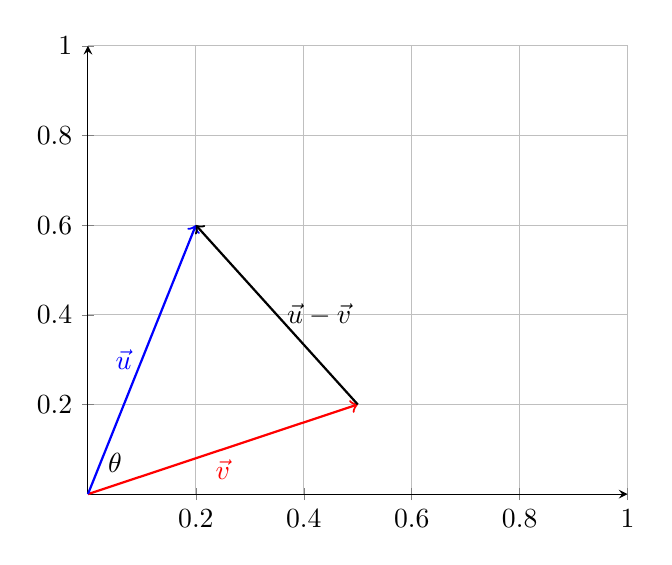
\begin{tikzpicture}
\begin{axis}[grid=major,axis x line=middle,
             axis y line=middle,
             after end axis/.code={
               \draw[red,thick,->] (axis cs:0,0) -- (axis cs:0.5,0.2) node[midway,below]{$\vec{v}$};
               \draw[blue,thick,->] (axis cs:0,0) -- (axis cs:0.2,0.6) node[midway,left]{$\vec{u}$}; 
               \draw[black,thick,->] (axis cs:0.5,0.2) -- (axis cs:0.2,0.6) node[midway,right]{$\vec{u} - \vec{v}$};
               \node at (axis cs:0.05,0.07){$\theta$};
  }]
\end{axis}
\end{tikzpicture}
\end{figure}
Let $\theta$ denote the angle between $\vec{u}$ and $\vec{v}$. Using the Law of Cosines, 
\[
\begin{aligned}
\norm{\vec{u} - \vec{v}}^2 &= (\vec{u} - \vec{v})\cdot(\vec{u} - \vec{v}) = \norm{\vec{u}}^2 + \norm{\vec{v}}^2 - 2\norm{\vec{u}}\norm{\vec{v}}\cos{\theta} \\
\norm{\vec{u}}^2 - 2(\vec{u}\cdot\vec{v}) + \norm{\vec{v}}^2 &= \norm{\vec{u}}^2 + \norm{\vec{v}}^2 - 2\norm{\vec{u}}\norm{\vec{v}}\cos{\theta} \\ 
&\to \boxed{\vec{u}\cdot\vec{v} = \norm{\vec{u}}\norm{\vec{v}}\cos{\theta}} \\
\end{aligned}
\]
This is the geometric definition of the dot product, which allows us to find the angle between two vectors easily.

\subsection{The Cauchy-Schwarz Inequality, Triangle Inequality}
\begin{theorem}[Cauchy-Schwarz Inequality]
If $\vec{u}$ and $\vec{v}$ are vectors in $\mathbb{R}^n$, then $|\vec{u}\cdot\vec{v}| \le \norm{\vec{u}}\norm{\vec{v}}$.
\end{theorem}

\begin{proof}
Rearranging the geometric definition of the dot product, we get $\cos{\theta} = \frac{\vec{u} \cdot \vec{v}}{\norm{\vec{u}}\norm{\vec{v}}}$. And since $|\cos{\theta}| \le 1$, we get that $ \left|\frac{\vec{u} \cdot \vec{v}}{\norm{\vec{u}}\norm{\vec{v}}}\right| \le 1 \to |\vec{u} \cdot \vec{v}| \le \norm{\vec{u}}\norm{\vec{v}}$.
\end{proof}

\begin{theorem}[Triangle Inequality]
If $\vec{u}$ and $\vec{v}$ are vectors in $\mathbb{R}^n$, then $\norm{\vec{u} + \vec{v}} \le \norm{\vec{u}} + \norm{\vec{v}}$.
\end{theorem}

\begin{proof}
\[
\begin{aligned}
\norm{\vec{u} + \vec{v}}^2 &= (\vec{u} + \vec{v})\cdot(\vec{u} + \vec{v}) \\
&= \vec{u}\cdot\vec{u} + 2(\vec{u}\cdot\vec{v}) + \vec{v}\cdot\vec{v} \\
&\le \norm{\vec{u}}^2 + 2|\vec{u}\cdot\vec{v}| + \norm{\vec{v}}^2  \\
\end{aligned}
\]
By Cauchy-Schwarz:
\[
\begin{aligned}
\norm{\vec{u} + \vec{v}}^2 &\le \norm{\vec{u}}^2 + 2\norm{\vec{u}}\norm{\vec{v}} + \norm{\vec{v}}^2 \\
&= (\norm{\vec{u}} + \norm{\vec{v}})^2 \\
\norm{\vec{u} + \vec{v}} &\le \norm{\vec{u}} + \norm{\vec{v}}
\end{aligned}
\]
\end{proof}

\subsection{Projections}
\begin{figure}[h!]
\centering
\begin{tikzpicture}
\coordinate (a) at (10,0);
\coordinate (b) at (2.5,3);
\coordinate (o) at (0,0);
\coordinate (c) at (2.5,0);
\draw[red,thick,->] (o) -- (a) node[midway,below]{$\vec{a}$};
\draw[blue,thick,->] (o) -- (b) node[midway,above]{$\vec{b}$};
\draw[green,->] (o) -- (c) node[midway,below]{$\proj_{\vec{a}}{\vec{b}}$};
\draw[dotted] (b) -- (c);
\node at (10.2,0) {$A$};
\node at (-0.2,-0.2) {$O$};
\node at (2.5,-0.2) {$C$};
\node at (2.7,3.2) {$B$};
\node at (0.5,0.2) {$\alpha$};
\end{tikzpicture}
\end{figure}

\end{document}
